%!TEX root = ../main.tex
\chapter{Page optimization}\label{ch:optimization}
In pursuing our goal to improve page load time so far, we have characterized the main bottleneck in a page load process on mobile devices. Our next step is to study the effect of optimizations on the page load time. There has been several industry tools that also study the page and suggest optimizations.
Google PageSpeed Insights \cite{pagespeedinsight} and Yahoo's YSlow \cite{yslow} are two noteable current web optimization platform. Although they both are trying to suggest optimizations to improve the overall web site's performance, but they suffer from some major problems.
Two main issues with Google PageSpeed Insights and Yahoo's YSlow solutions are as follows:
 \begin{itemize}
  \item They do not directly measure the benefit of an optimization on the page load time. Instead, they use a scoring mechanism that do not necessarily correlate well with the real page load improvements.
  \item They are using fixed set of rules and do not consider optimizing for each particular case.\\
   
\noindent For example, PageSpeed Insights encourages users to inline (small) scripts in the HTML source file to avoid additional roundtrip times.
On the contrary,  YSlow recommends to make Javascript and CSS scripts external, to benefit from possible caching. This differences arise because of not considering the varying nature of servers, clients and network connections.\\
\noindent We should also note that modification do not always help.
For example, a popular improvement to reduce the download time is enabling compression in server side. Modern browsers support this feature automatically and decompress the received objects. Although this technique seems to be always beneficial, one should be careful about the gain achieved in reducing download time against increased computing time needed to decompress the whole session.
\end{itemize}

\noindent In this chapter, first, we study current web page optimization solutions, mainly Google's PageSpeed Insights and Yahoo's YSlow . Then we analyze these optimizations and study their effect on page load time using our testbed.

\noindent We then, illustrate building blocks of our future platform which scores each optimization based on it's contribution to the page load time. Having a platform that shows the effects of optimizations on page load time and considers the dynamic nature of servers, clients and network connections at the same time, would enable us to more precisely suggest customized optimizations for each particular case.
\section{Current page optimization solutions}
\subsection{Google's PageSpeed Insights}
PageSpeed Insights \cite{pagespeedinsight} is a tool that helps developers optimize their web pages by analyzing the pages and generating tailored suggestions to make the pages faster.
PageSpeed Insights measures the performance of a page for mobile devices and desktop devices. It fetches the URL twice, once with a mobile user-agent, and once with a desktop-user agent. PageSpeed Insights analysis does not use real devices. It fetches a site with a webkit renderer (the same rendering engine that powers Chrome and Safari) that emulates both mobile device and desktop devices.\\

\noindent The PageSpeed Score ranges from 0 to 100 points. The higher the score, the better the performance. However, since the performance of a network connection varies considerably, PageSpeed Insights only considers the network-independent aspects of page performance: the server configuration, the HTML structure of a page, and its use of external resources such as images, JavaScript, and CSS. Implementing the suggestions should improve the relative performance of the page. However, the absolute performance of the page will still be dependent upon a user's network connection.\\\\

\subsubsection{Architecture:}
Developer makes a simple HTTP request to google PageSpeed Insights servers and gives a URL to fetch. PageSpeed Insights will fetch and render that URL, then runs the Page Speed library on it and gives back the result as depicted in figure \ref{fig:pagespeed}
\begin{figure}[!htb]
\centering{
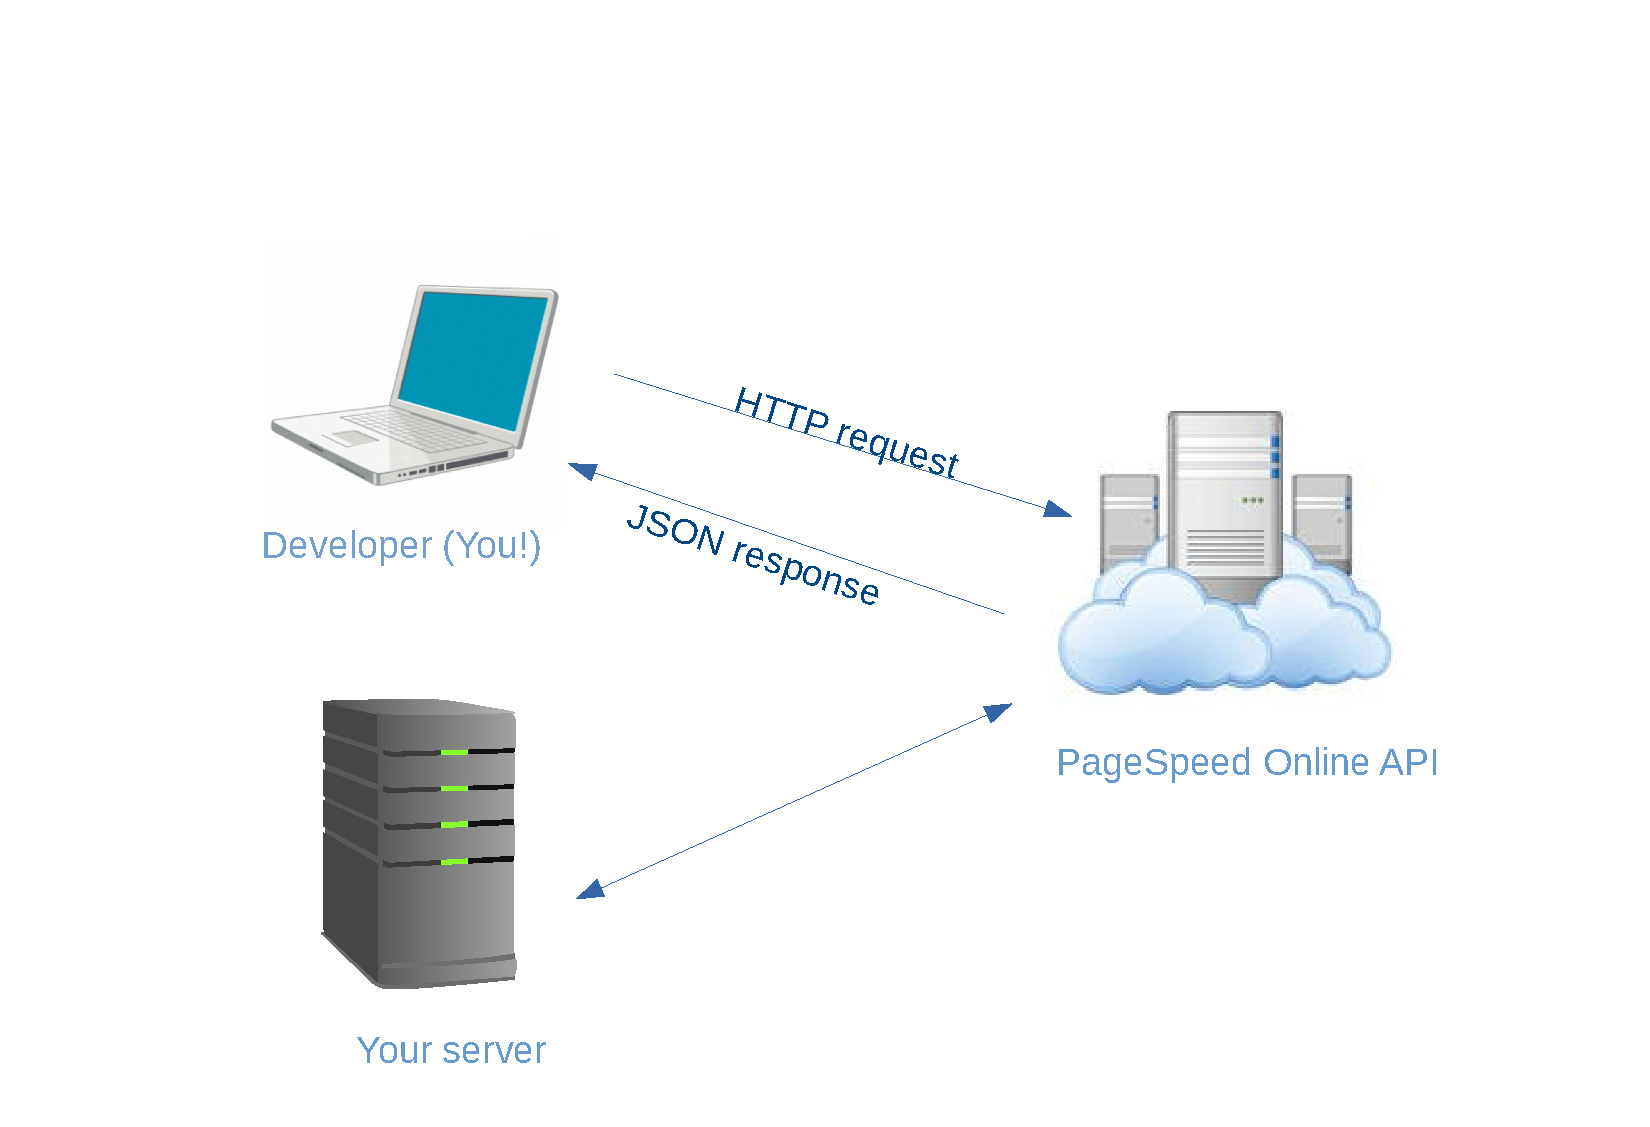
\includegraphics[scale=0.5]{./figures/optimization/pagespeed.pdf}
\caption{PageSpeed Insights online API}
\label{fig:pagespeed}
}
\end{figure}

\subsubsection {PageSpeed SDK}
A webpage is fetched and rendered using {\em pagespeed\_webkit} and then the defined rules  in {\em lib/trunk/src/pagespeed/rules} are applied and the formatted results are presented.\\
Results of all the rules are presented to the user. Each PageSpeed rule generates an impact number (an unbounded floating point value) that indicates the importance or priority of implementing the rule-result suggestions for the rule, relative to other rules.\\

\noindent For instance, if enabling compression would save 1MB, while optimizing images would save 500kB, the {\em "Enable Compression"} rule would have an impact value that is twice that of the {\em "Optimize Images"} rule. An impact of zero indicates that there is no suggestion for improvement for that rule.
Following is a code snippet of a sample response of PageSpeed Insights API:
\begin{minted}[frame=leftline, framerule=1.5pt, rulecolor=\color{blue}]{json}
{
 "kind": "pagespeedonline#result",
 "id": "/speed/pagespeed",
 "responseCode": 200,
 "title": "PageSpeed Home",
 "score": 90,
 "pageStats": {
  "numberResources": 22,
  "numberHosts": 7,
  "totalRequestBytes": "2761",
  "numberStaticResources": 16,
  "htmlResponseBytes": "91981",
  "cssResponseBytes": "37728",
  "imageResponseBytes": "13909",
  "javascriptResponseBytes": "247214",
  "otherResponseBytes": "8804",
  "numberJsResources": 6,
  "numberCssResources": 2
 },
   "comment": "..."
   "MinifyJavaScript": {
    "localizedRuleName": "Minify JavaScript",
    "ruleImpact": 0.1417,
   "comment": "..."
 }
}
\end{minted}
The improvements/fixes shown on PageSpeed Insights are sorted in decreasing order of their {\em "Rule Impact"} value. The one that has more Impact value will be shown first, which means that fixing it would have significant improvement in webpage performance.
\subsubsection{ Effect of PageSpeed Insights' rules on page load time}
Goal of these experiments is to see how much effect the suggestions of PageSpeed Insights has on page load time. For this purpose, we have considered 5 websites for which PageSpeed suggests to Inline JS/CSS, Minify HTML/CSS/JS and Optimize images. For each website, entire website is downloaded locally on testbed and modified to implement three suggestions; Inlining, minification and optimizing images separately to see the impact of each change on page load times. \\
\noindent We performed these experiments with three different network profiles b1-d50, b5-d50 and b20-d50 where "b" stands for bandwidth and "d" stands for delay. Results for b20-d5- are only shown here.

\begin{enumerate}
\item {\textbf {Inlining:}}\\
PageSpeed Insights suggests to inline only specific JS/CSS. Inlining should ideally help to reduce overall page load time, specifically total download time.
Experiments were done with 4 websites of which inlining actually helped two and didn't help other two as shown in figure \ref{fig:InsightsInlining_b20_d50} . For first two sites page load time did not improve; in fact, worsened.

\begin{figure}[!htb]
  \centering
    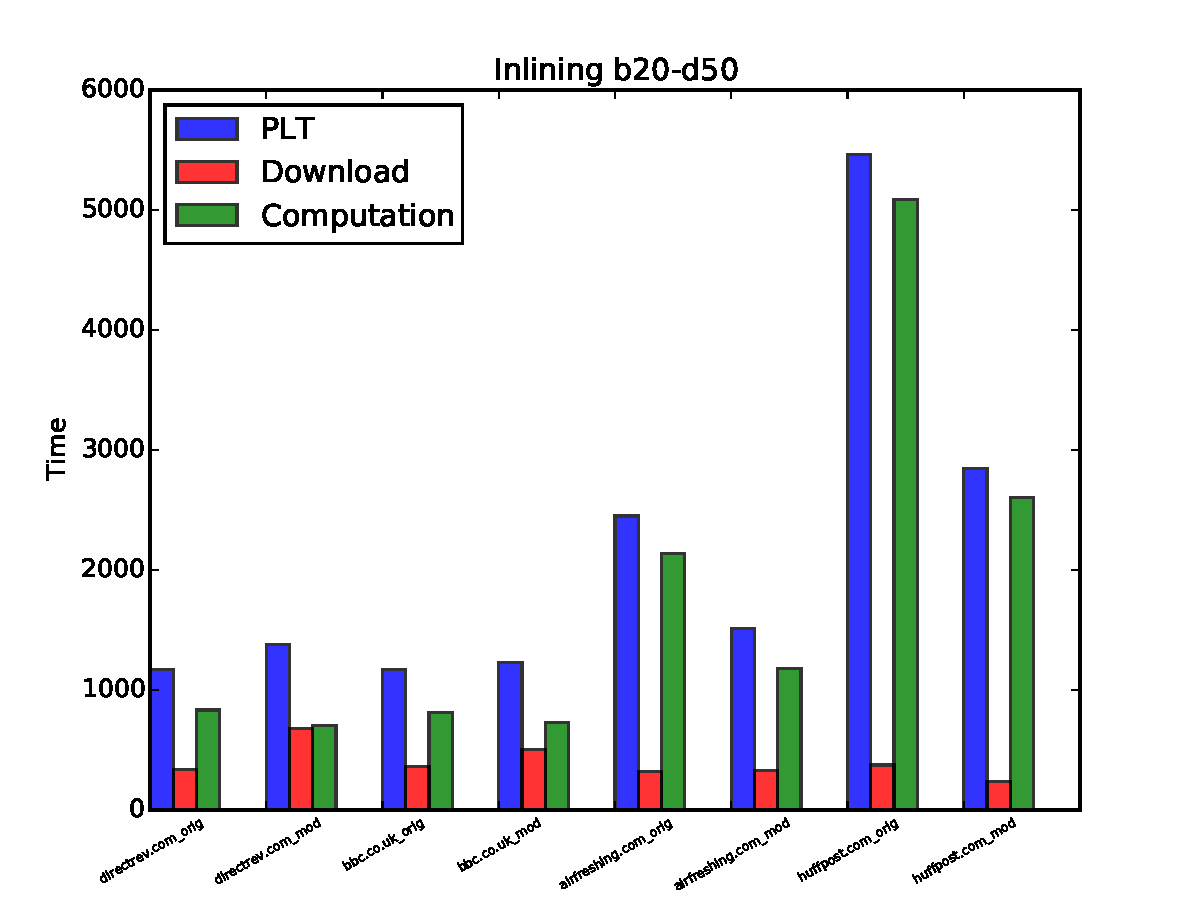
\includegraphics[width=0.85 \textwidth]{./figures/optimization/InsightsInlining_b20_d50.pdf}
  \caption {Page load time before/after inlining using PageSpeed insights }
  \label{fig:InsightsInlining_b20_d50}
\end{figure}

% add more explanation

\item  {\textbf {Optimize Images:}}\\
PageSpeed Insights suggests to optimize few images so that their size is reduced which should eventually help reducing page load time. One disadvantage to this suggestion is size reduction is at the cost of high quality. Compressing images results in low quality which can affect user experience.\\

As we observe from figure \ref{fig:InsightsOptimizeImages_b20_d50}, optimizing images, helps to reduce page load time for {\em huffpost.com} and {\em airfreshing.com} while does not help in {\em youku.com} and {\em directrev.com} and even hurts in {\em bbc.co.uk}.
\begin{figure}[!htb]
  \centering
    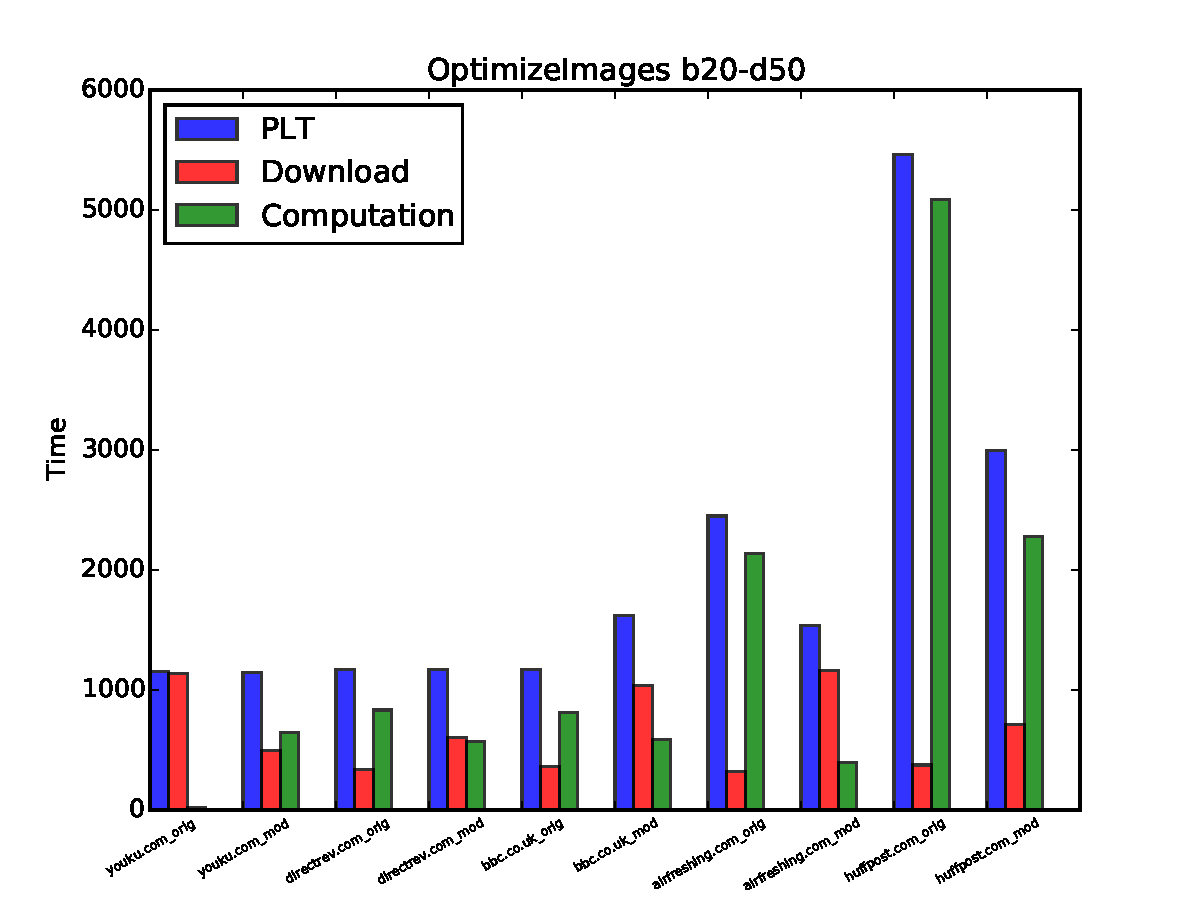
\includegraphics[width=0.85 \textwidth]{./figures/optimization/InsightsOptimizeImages_b20_d50.pdf}
  \caption {Page load time before/after optimizing images using PageSpeed insights }
  \label{fig:InsightsOptimizeImages_b20_d50}
\end{figure}

\item {\textbf{Minification:}}\\
Page speed Insights suggests to minfiy JS/CSS/HTML to reduce the size of those files so that download time is reduced and page load time is improved. As shown in figure  \ref{fig:InsightsOptimizeImages_b20_d50}, minifcation alone is not always helping to reduce page load time. We can see again, minification has helped {\em directrev.com }, {\em airfreshing.com} and {\em huffpost.com} but, hurt {\em youku.com} and {\em bbc.co.uk}.
\begin{figure}[!htb]
  \centering
    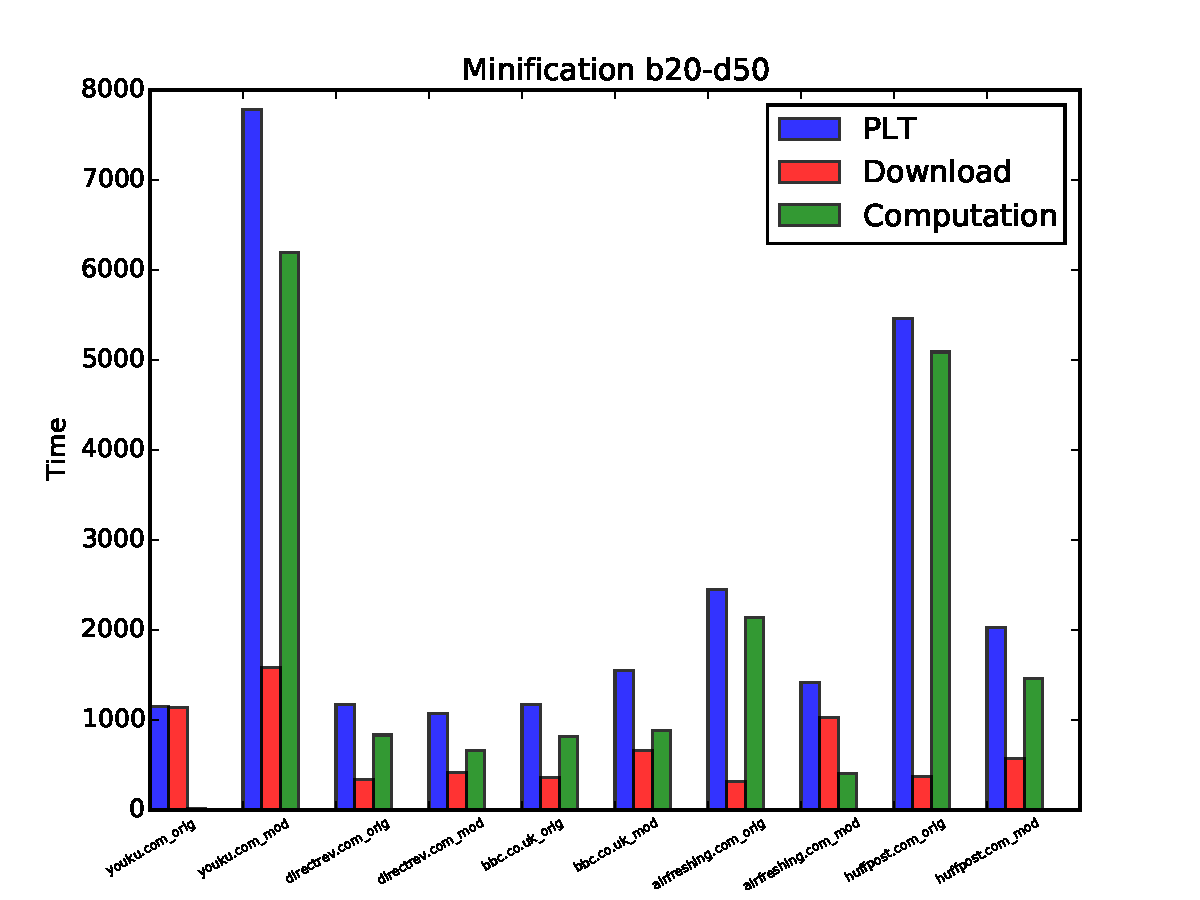
\includegraphics[width=0.85 \textwidth]{./figures/optimization/InsightsMinification_b20_d50.pdf}
  \caption {Page load time before/after Minification using PageSpeed insights }
  \label{fig:InsightsMinification_b20_d50}
\end{figure}

\end{enumerate}

\subsection{Yahoo's YSlow}
Yahoo's YSlow \cite{yslow}  grades web page based on one of three predefined ruleset or a user-defined ruleset.
It also offers suggestions for improving the page's performance and provides tools for performance analysis.\\

\noindent YSlow works in three phases to generate its results.

\begin{enumerate}

\item YSlow crawls the DOM to find all the components (images, scripts, stylesheets, etc.) in the page. After crawling the DOM, YSlow loops through Firebug's \cite{firebug} Net Panel components and adds those to the list of components already found in the DOM.
\item YSlow gets information about each component: size, whether it was gzipped, Expires header, etc. YSlow gets this information from Firebug's Net Panel if it's available. If the component's information is not available from Net Panel (for example, the component was read from cache or it had a 304 response), YSlow makes an XMLHttpRequest to fetch the component and track its headers and other necessary information.
\item YSlow takes all this data about the page and generates a grade for each rule, which produces the overall grade.
\end{enumerate}

\noindent Figure \ref{fig:yslow_stonybrook} shows a sample analysis for {\em www.cs.stonybrook.edu} using YSlow.
\begin{figure}[!htb]
  \centering
    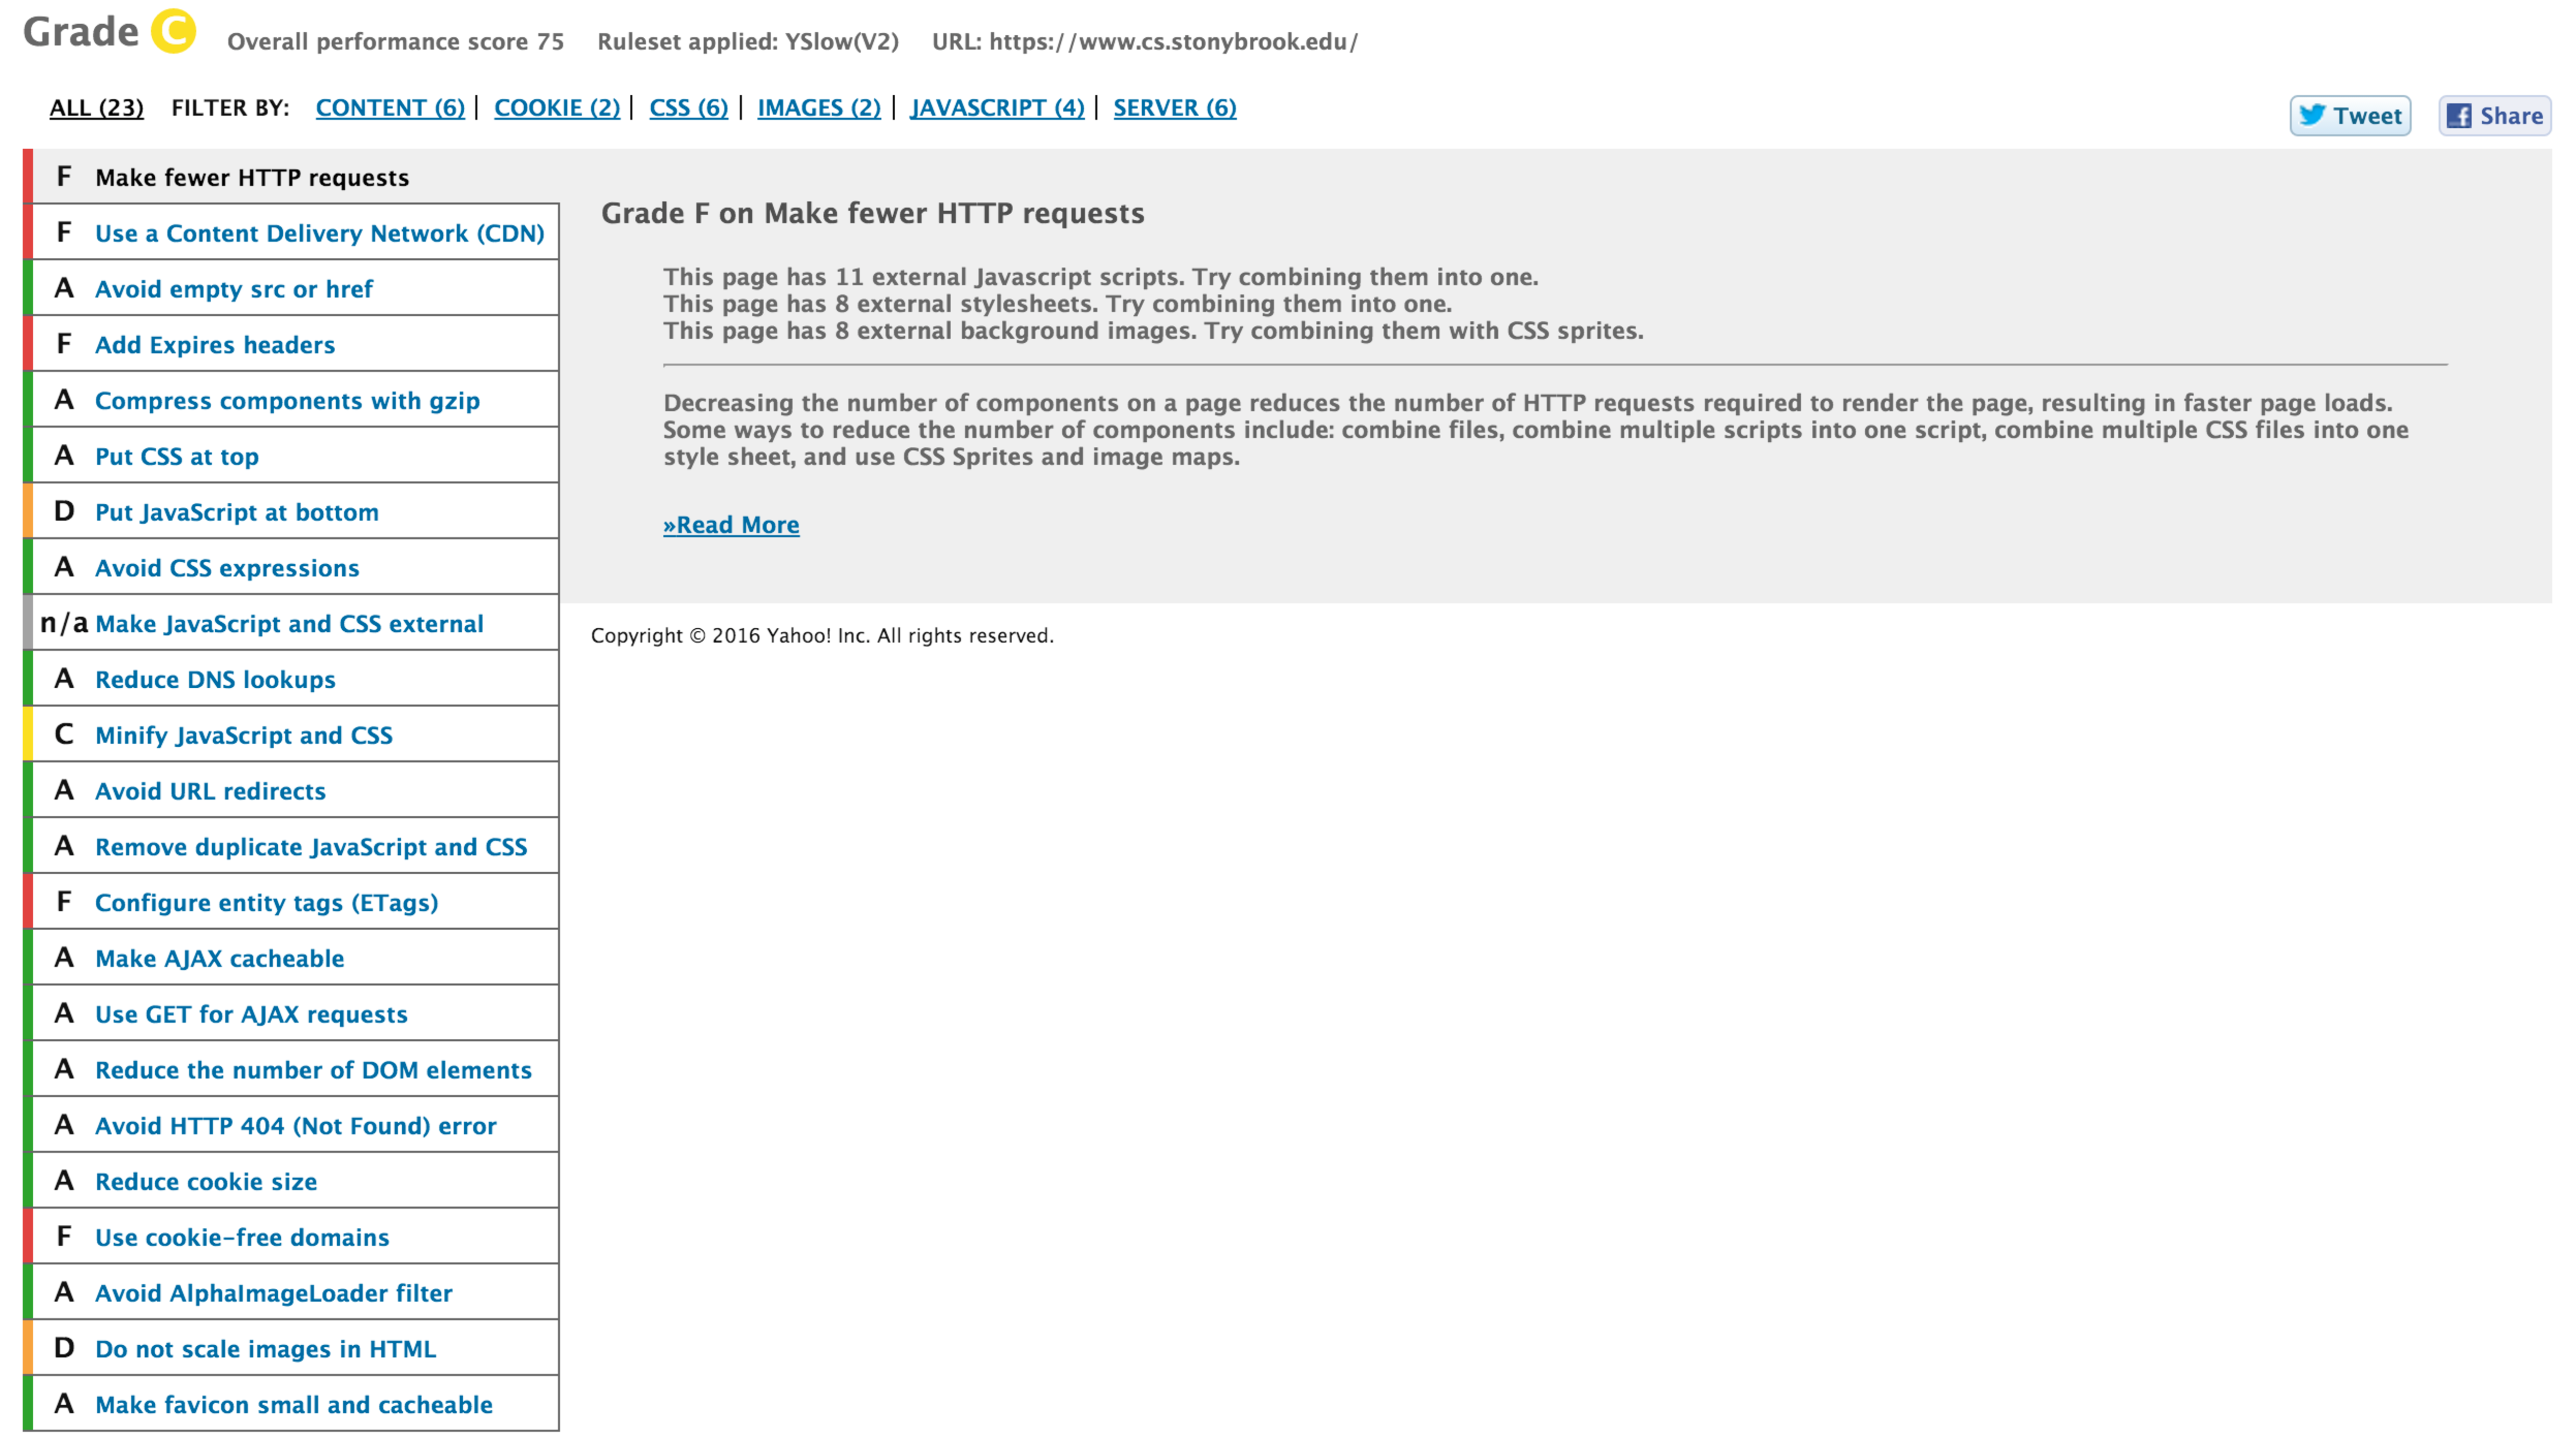
\includegraphics[width=0.85 \textwidth]{./figures/optimization/yslow_stonybrook.pdf}
  \caption {Sample YSLOW analysis for {\em www.cs.stonybrook.edu}}
  \label{fig:yslow_stonybrook}
\end{figure}

\noindent Since YSlow share the same problems with Google's PageSpeed Insight's(Fixed rule sets and unrealistic weights), the optimization results would be similar to the PageSpeed's Insights results.

\section{Our Approach: PLTSpeed}
\noindent In this section, we briefly discuss our approach in which we will score each optimization based on it's contribution to the page load time. We also take into account different network and client conditions when suggesting an optimization.

\subsection{A framework to predict page load time}
 As we have discussed earlier (\S\ref{ch:methodology}), WProf can capture the various activities performed during page load. We analyze these capture files to generate a JSON file for each page load process. Each JSON file contains the timing for all objects in a web page along with their dependencies. A sample snippet of such a JSON file is shown below.
 

 
 \begin{minted}[frame=leftline, framerule=1.5pt, rulecolor=\color{blue}]{json}

 {
   "n_download_no_trigger" : 1,
   "start_activity" : "download_0",
   "name" : "original.testbed.localhost_test4.html",
   "load_activity" : -1,
   "objs" : [
      {
         "when_comp_start" : 1,
         "url" : "http://original.testbed.localhost/test4.html",
         "id" : "r1",
         "comps" : [
            {
               "s_time" : 59.6280004829168,
               "time" : 12.5759998336435,
               "id" : "r1_c1",
               "type" : "evalhtml",
               "e_time" : 72.2040003165603
            },
            {
               "s_time" : 75.6310001015663,
               "time" : 0.867000780999703,
               "type" : "evalhtml",
               "id" : "r1_c2",
               "e_time" : 76.498000882566
            }
         ],
         "download" : {
            "receiveFirst" : 2,
            "len" : 295,
            "dns" : 0,
            "dnsEnd" : -1,
            "receiveHeadersEnd" : 9,
            "sslEnd" : -1,
            "connectEnd" : 6,
            "connectStart" : 0,
            "id" : "download_0",
            "receivedTime" : "11.2190004438162",
            "sslStart" : -1,
            "dnsStart" : -1,
            "receiveLast" : 2.21900044381618,
            "s_time" : 0,
            "sendEnd" : 7,
            "sendStart" : 6,
            "type" : "text/html"
         }
      }
 \end{minted}

 
 
\noindent These JSON files can be seen as structured representation of the whole page load. Now, if we apply an optimization to a Web page, the resulting JSON file will reflect the result of the applied optimization along with new timings and dependencies.\\

\noindent If we had access to the new timings beforehand, we could rewrite the original JSON file and produce the new JSON file. In other words, if we could predict the new computation and download time for each activity involved in a page load process, we were able to rewrite the original JSON file and predict the new page load time after optimizations has been applied.
This process is illustrated in figure \ref{fig:platform}.
\begin{figure}[!htb]
  \centering
    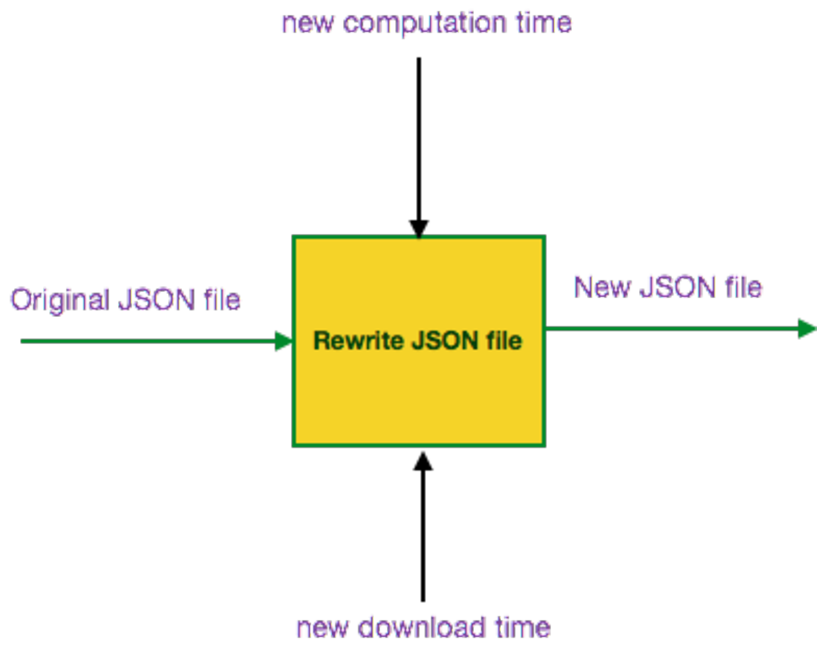
\includegraphics[width=0.85 \textwidth]{./figures/optimization/platform.pdf}
  \caption {Rewriting the original JSON file to predict new page load time.}
  \label{fig:platform}
\end{figure}

\noindent We process each of these new generated JSON files and calculate the critical rendering path. The length of the critical path is the page load time.\\

\subsection {The prediction engine}
To complete our framework from previous section, we now need an infrastructure to predict computation and download times after a certain parameter is changed. This parameter can be applying a new optimization or just a change in connection bandwidth.
 
\noindent For example, to predict new download time after a certain optimization is applied to a Web page, in our testbed, we can apply optimization to lots of locally served web pages. By actually running experiments before and after that optimization, we will be able to model download time for each object present in a page structure.\\
\noindent This model can predict the future network/computation time for each object. This feature (As discussed in previous section) enables us to manipulate the original JSON file and calculate the new critical rendering path time for a particular Web page without applying that particular optimization.

\noindent The block diagram for predicting new download times is depicted in figure \\\ref{fig:predictionengine} 

\begin{figure}[!htb]
  \centering
    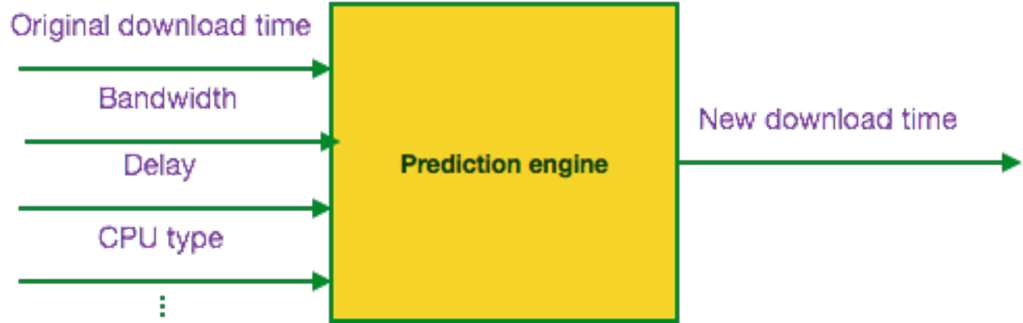
\includegraphics[width=0.85 \textwidth]{./figures/optimization/predictionengine.pdf}
  \caption {Prediction engine}
  \label{fig:predictionengine}
\end{figure}

\noindent We walk through an example to see how computation/networking time can be modeled for a certain type of modification.\\
We apply minification to an external CSS/Javascript and use our testbed to model the impact of this modification. "Minification is the process of removing all unnecessary characters from source code without changing its functionality"\cite{wiki_minification}. \\
The experiment is set up to run an emulated 4G connection. We use Alexa's top 200 web sites and in this case, experiments are run in a desktop environment.
To ignore already minified scripts, we use a simple heuristic which looks for white spaces in the beginning of script source file. If there is no white space, we consider that script as "already minified".\\
The goal is to model computation and network time for minified scripts. We have the timing for all objects in the original web page. Using the testbed, we also have access to the timing for all objects in the new modified web page. This new modified web page has all of it's scripts minified. In order to model how minification affects the computation and networking time, we use linear regression modeling as our prediction algorithm.\\
\noindent In figure \ref{fig:afterbeforeoncp}, the gray bars are length of the original {\em www.youtube.com} (before minification) and the color bars are for minified {\em www.youtube.com}. As we can observe, minification reduces length of objects on critical path in this case and leads to a decreased page load time.
\begin{figure}[!htb]
  \centering
    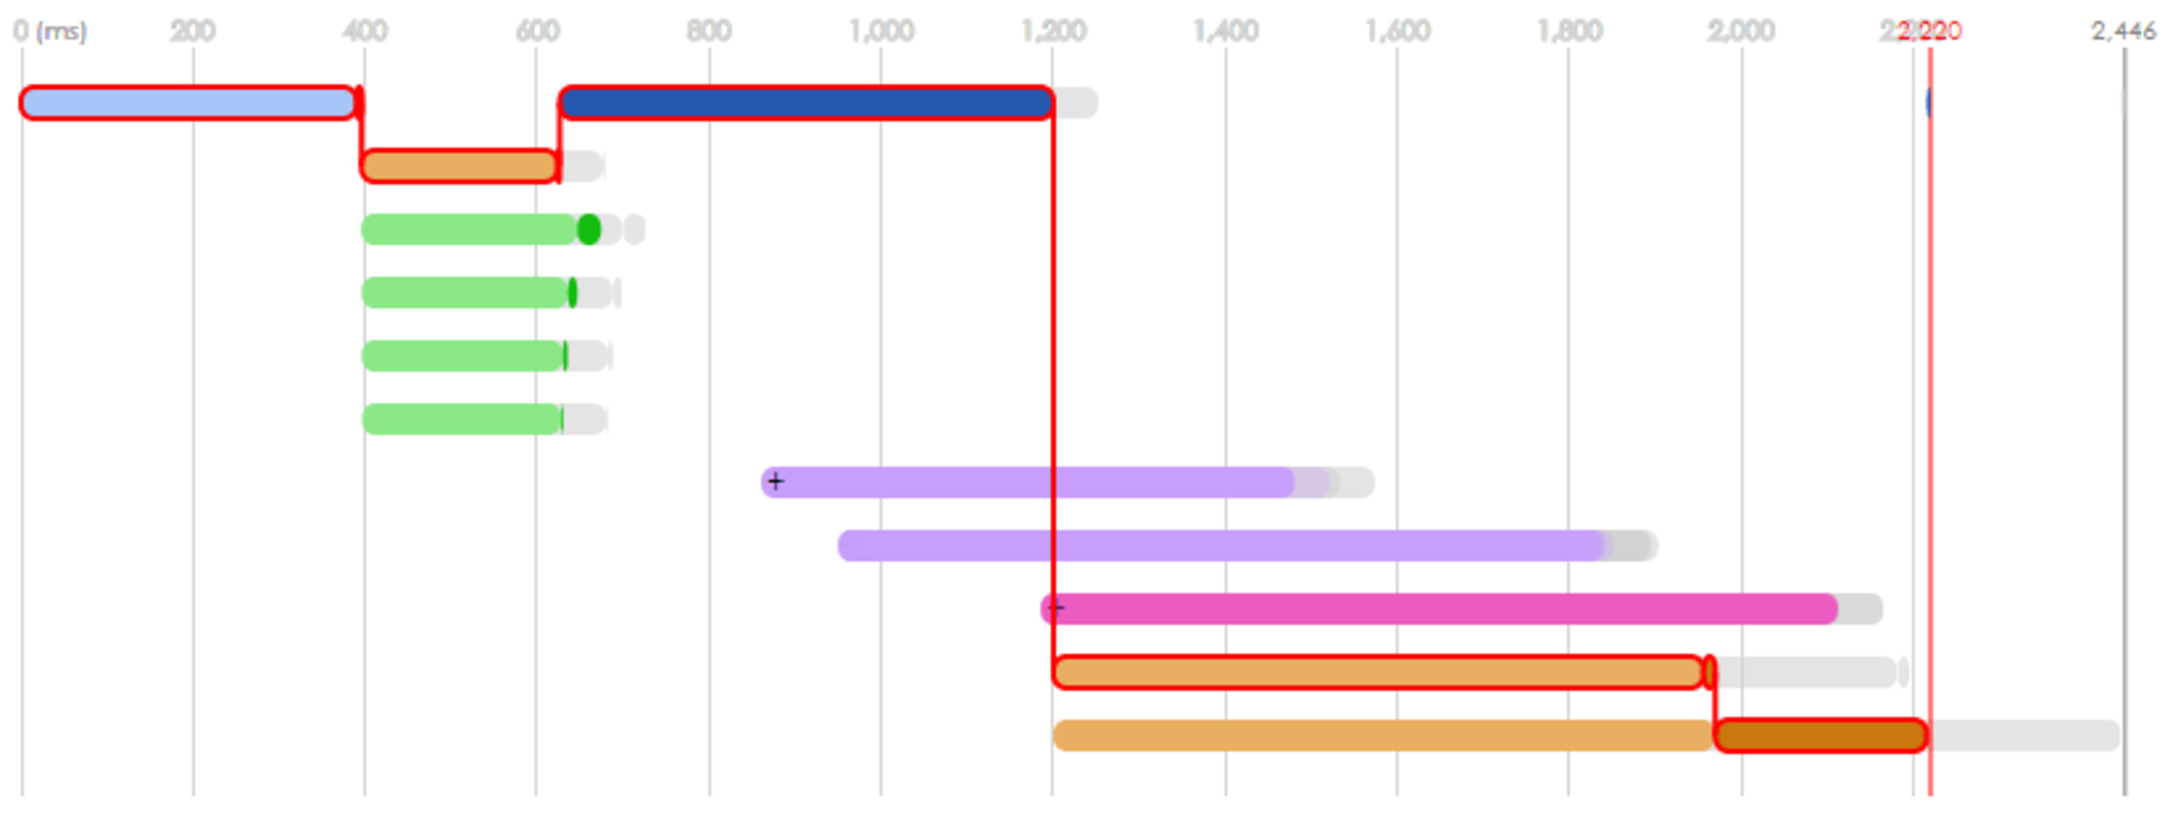
\includegraphics[width=0.85 \textwidth]{./figures/optimization/afterbeforeoncp.pdf}
  \caption {Page load time before/after minification on www.youtube.com}
  \label{fig:afterbeforeoncp}
\end{figure}

\subsection {Future work}
After completing our framework to predict page load time, in future, we will build a web based platform that suggests to users best optimizations applicable to their Web sites. This platform will consider optimization's contribution to page load time along with different networking conditions and user setups.\\
\noindent  One should note that when combining optimizations, the whole gain/loss will not be equal to the sum of all optimizations. Hence, part of our future job will be to study the effect of combination of optimizations. For example, we may observe that minification alone, will improve page load time by 10\% and inlining improves the page load time by 5\% in a certain environment. Obviously we can not conclude that when minification and inlining are both applied to a Web page, we will see overall 15\% improvement in page load time.

%Here we can add d3.js figures for original and modified pages.(Meghna's plots)
